\documentclass[letterpaper,12pt]{article}
\usepackage[top=1in, left=1.25in, right=1.25in, bottom=1in]{geometry}
\usepackage[utf8]{inputenc}
\usepackage[T1]{fontenc}
\usepackage[spanish]{babel}
\usepackage{graphicx}
\usepackage{caption}
\usepackage{float}
\usepackage[backend=biber,style=numeric,sorting=none]{biblatex}
\usepackage{amsmath}
\addbibresource{bib/referencias.bib}
\usepackage{subcaption}
\usepackage{fancyhdr}
\pagestyle{fancy}
\lhead{Reporte del Proyecto 2}
\rhead{Programación Orietada a Objetos}

\begin{document}

\tableofcontents
\clearpage

\section{Introducción}

\begin{itemize}
\item \textbf{Planteamiento del Problema:} Se busca diseñar un programa que permita representar dos tipos de empleado con características y operaciones principales compartidas, como el nombre del empleado, su apellido y su seguro social; así como características únicas para cada tipo de empleado, como su forma de pago, empaquetando los códigos para organización.

\item \textbf{Motivación:} La implementación de este código permitirá poner en practica la creación de una clase padre planeada desde un inicio para tener hijos siendo una clase abstracta, permitiendo implementar y practicar nuestros conocimientos en la creación de clases con herencia, sobrescritura y el polimorfismo; así como acostumbrándonos a empaquetar por formalidad y estructura y a la ejecución de códigos empaquetados.

\item \textbf{Objetivos:} Implementar un programa en Java que mediante el uso de una sola referencia a una clase padre abstracta, se manejen diferentes tipos de empleados utilizando polimorfismo y herencia, mostrando en cada caso las características que tiene cada empleado. Asimismo se busca empaquetar las clases utilizadas, permitiendo manejar los archivos ordenadamente.


\end{itemize}
\section{Marco Teórico}
    \begin{itemize}

    \item \textbf{Encapsulamiento: }El \textit{Encapsulamiento} es el principio de restringir el acceso directo a los atributos de una clase, de modo que solo puedan ser modificados mediante métodos controlados como getters y setters. Este enfoque nos ayuda a proteger los datos, evita inconsistencias y brinda mayor control del programa.~\cite{Encapsulamiento}
    
    \item \textbf{Paquetes} Son el mecanismo que usa Java para facilitar la modularidad del código. Un paquete puede contener una o más definiciones de interfaces y clases, distribuyéndose habitualmente como un archivo. Para utilizar los elementos de un paquete es necesario importar este en el módulo de código en curso, usando para ello la sentencia \textbf{import}. ~\cite{Paquetes}
    
    \item \textbf {Herencia:} Es un concepto que permite definir nuevas clases basadas en clases ya existentes, aprovechando y extendiendo su funcionalidad, reutilizando código. Para heredar una clase a otra, se usa la palabra reservada \textbf{extends} al declarar la clase. ~\cite{HerenciaPolimorfismo}

    \textbf{Abstracción: }Es la capacidad de representar problemas complejos de una forma mas simple, dejando solo las caracteristicas escenciales y ocultando los detalles innecesarios. ~\cite{ClasesAbstractasInterfaces}
    
    \textbf {Clases abstractas e interfaces: }Las clases abstractas son un tipo de clases de las cuales no se puede crear un objeto a partir de ellas; una clase abstracta puede contener métodos abstractos, que indican que se deben implementar en la clase que herede, o métodos con comportamiento ya definido; la forma en la que se crea una clase abstracta es usando la palabra reservada \textbf{abstract}.

    Una interfaz es un modelo del que tampoco se pueden crear objetos. Contiene solo métodos abstractos y atributos constantes estáticos, por lo que las clases que usen esta interfaz tienen la obligación de implementar todos los metodos heredados. Para crear una interfaz, es con la palabra reservada \textbf{interface} y para usarla con \textbf{implements}. ~\cite{ClasesAbstractasInterfaces}
        
    \item \textbf{Polimorfismo: }Es la capacidad de un objeto para adquirir diferentes comportamientos, mas específicamente, es el concepto de implementar métodos con el mismo nombre pero distinto comportamiento. ~\cite{HerenciaPolimorfismo}
    
\end{itemize}

\section{Desarrollo}

Para este proyecto se ha implementado el polimorfismo de una clase abstracta, sobrescritura de métodos y comunicación con el constructor de la clase base.

Todas las clases han sido empaquetadas siguiendo la sintaxis del \textbf{fullQualifiedName}: \textbf{/mx/unam/fi/poo/py2/}, agregando: \textbf{package mx.unam.fi.poo.py2;} al inicio de cada clase.\\

Comenzamos creando la clase abstracta \textbf{Empleado} que tiene los atributos privados \textbf{nombre, apellido y seguroSocial}, datos que el constructor recibe y llama a los métodos \textbf{setters} de cada atributo, además se generaron sus respectivos \textbf{getters}. Empleado tiene el método abstracto \textbf{ingresos} que se sobrescribirá en cada clase hija.
También contiene el método sobrescrito \textbf{toString} que imprime los atributos en determinado formato.\\

La clase \textbf{EmpleadoPorComision}, heredada de la clase \textbf{Empleado}, tiene los atributos privados \textbf{tarifa} y \textbf{ventas}. Su constructor se comunica con el constructor de la clase base con la palabra reservada \textbf{super}, asignandole los valores corresponfientes; además, el contructor asgina los atributos propios de esta clase. 

Para los \textbf{setters} de los dos atributos, hicimos la validación para que la tarifa de venta quede estrictamente entre 0 y 1 en el caso de \textbf{tarifa}, y para \textbf{ventas} validamos que la cantidad sea mayor a 0. 

Después tenemos los métodos sobrescritos \textbf{toString} y \textbf{ingresos}. El primero extiende la implementación de \textbf{toString} de la clase base y además imprime los nuevos atributos siguiendo el formato ya creado. El segundo método multiplica las tarifas y las ventas para obtener un total de ingresos obtenidos.\\

La clase \textbf{EmpleadoAsalariado}, heredada de la clase \textbf{Empleado}, contiene el atributo privado \textbf{salarioSemanal}. Similar a la clase anterior, su constructor se comunica con el constructor de la clase base con \textbf{super}, recibiendo los atributos correspondientes; también el constructor asigna los atributos de su propia clase. 

En \textbf{setSalarioSemanal} simplemente validamos que el salario sea mayor a 0. Igualmente tenemos los métodos sobrescritos \textbf{toString} e \textbf{ingresos}. El primero funciona de la misma manera que el de la clase anterior, sin embargo, este imprime también al atributo \textbf{salarioSemanal} en el formato ya acordado. El segundo método obtiene el salario mensual, al multiplicar \textbf{salarioSemanal} por 4.\\

Finalmente para la clase \textbf{MainApp}, en método \textbf{main} comenzamos creando una referencia polimórfica de tipo \textbf{Empleado}, la cual se 'transforma' en diferentes tipos de empleado a lo largo del programa. Para hacerlo más evidente, fuimos intercalando entre \textbf{EmpleadoPorComision} y \textbf{EmpleadoAsalariado}. Para cada empleado, se imprimen sus métodos \textbf{toString} e \textbf{ingresos}, mostrando las características de cada empleado.  

\section{Diagramas UML}

\begin{figure}[H]
    \centering
    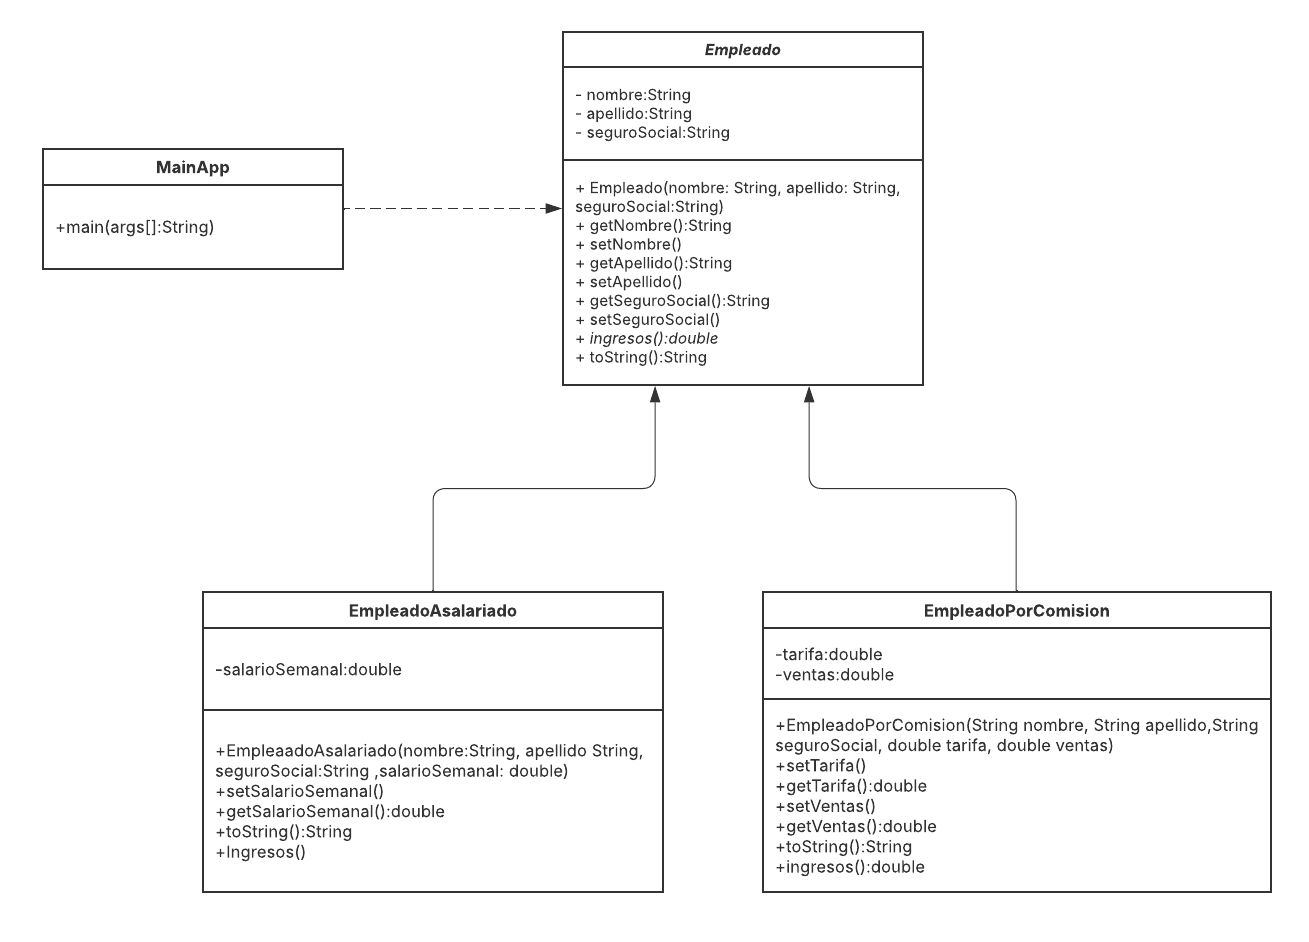
\includegraphics[width=\linewidth]{Imagenes/Clase UML.png}
    \caption*{Diagrama UML de Clases}
\end{figure}
\begin{figure}[H]
    \centering
    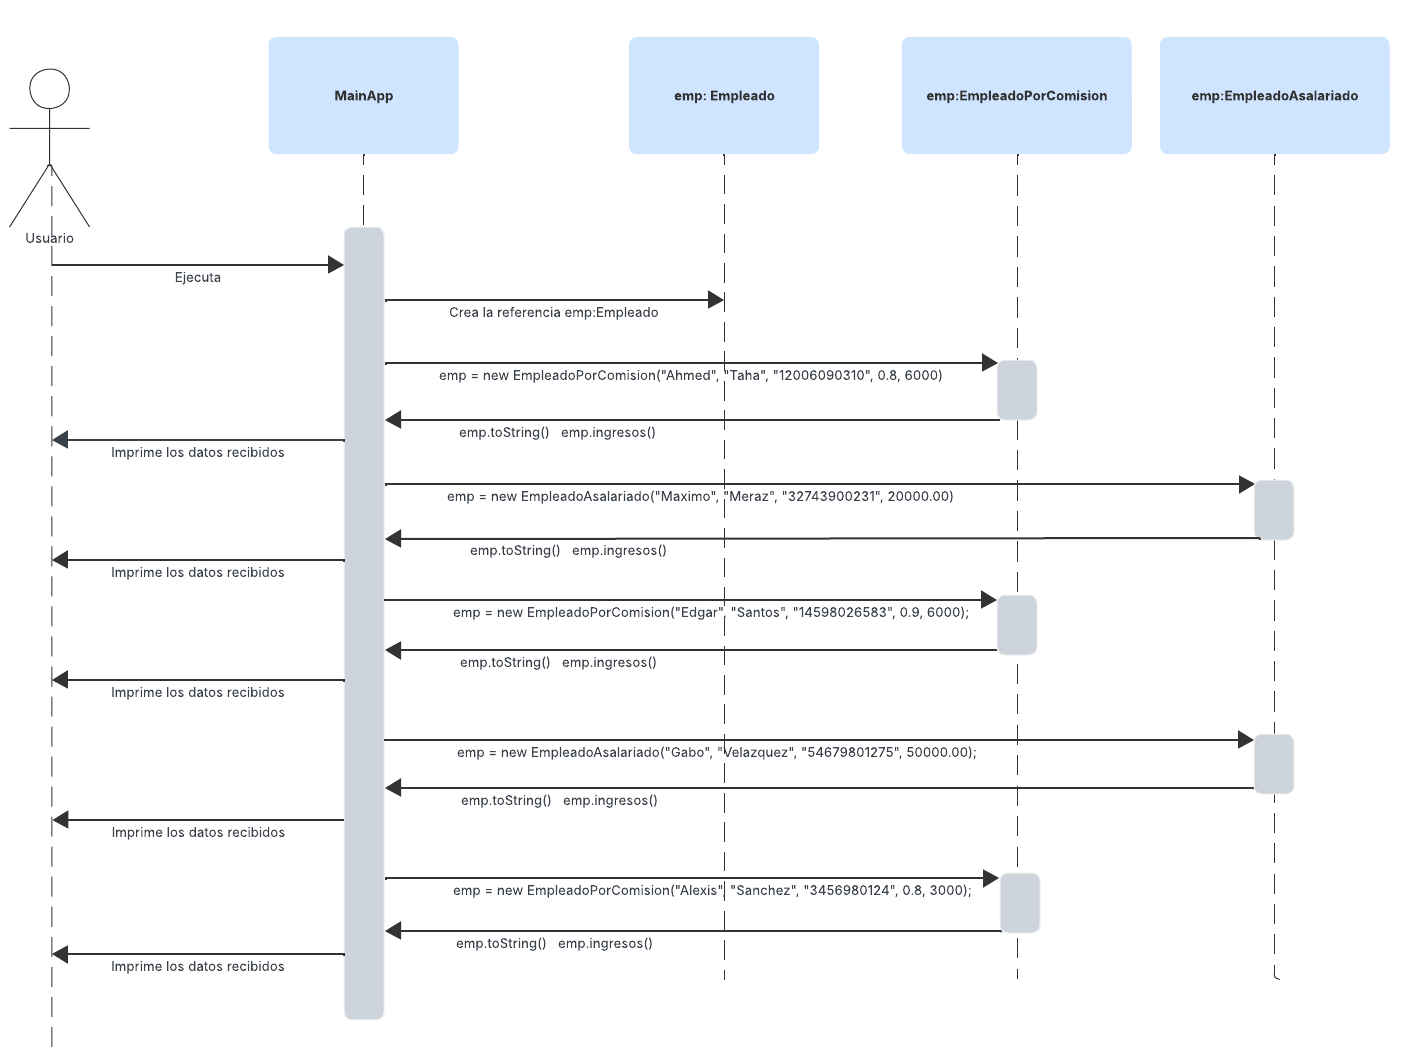
\includegraphics[width=\linewidth]{Imagenes/Diagrama de secuencia.png}
    \caption*{Diagrama UML de Secuencia}
\end{figure}

\section{Resultados}

\begin{figure}[H]
    \centering
    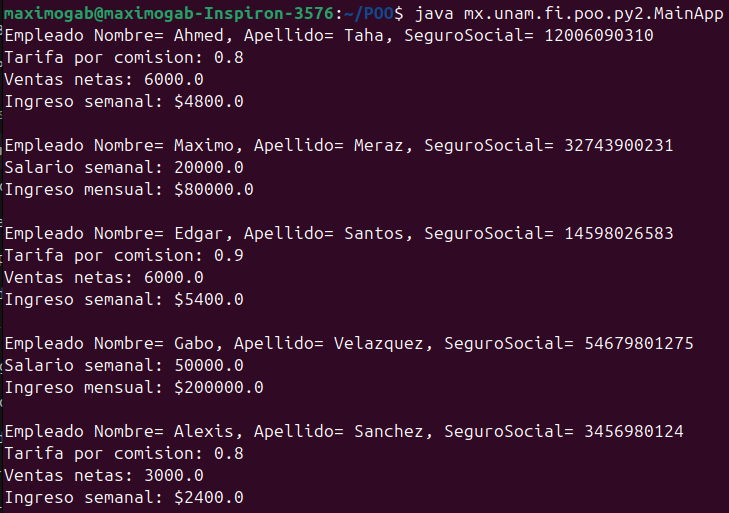
\includegraphics[width=0.8\linewidth]{Imagenes/Resultado.png}
\end{figure}


\section{Conclusiones}
El desarrollo de este proyecto permitió consolidar y aplicar de manera práctica conceptos de la Programación Orientada a Objetos, así como es la herencia para reutilizar código, las clases abstractas para definir un 'esqueleto' o súperclase común, la sobrescritura de métodos para especializar comportamientos en las clases derivadas, y el polimorfismo mediante referencias de la clase base abstracta \textit{Empleado},permitiendo manipular objetos de distintos tipos desde una misma referencia. 

En esta practica, comprendimos la importancia que tiene la comunicaciones entre clases, así como la organización de varios archivos dentro de un mismo paquete para mantener un orden y estructura correcta. Este trabajo nos permitió integrar los principios de POO en un proyecto con un entorno bien estructurado.
 
\printbibliography

\end{document}